\documentclass{article}

\usepackage{geometry}
\usepackage{amsmath}
\usepackage{graphicx, eso-pic}
\usepackage{listings}
\usepackage{hyperref}
\usepackage{multicol}
\usepackage{fancyhdr}
\usepackage{xcolor}
\pagestyle{fancy}
\fancyhf{}
\hypersetup{ colorlinks=true, linkcolor=black, filecolor=magenta, urlcolor=cyan}
\geometry{ a4paper, total={170mm,257mm}, top=40mm, right=20mm, bottom=20mm, left=20mm}
\setlength{\parindent}{0pt}
\setlength{\parskip}{0.3em}
\renewcommand{\headrulewidth}{0pt}
\rfoot{\thepage}
\lfoot{Seleksi IEEEXtreme 15.0 ITB}
\lstset{
    basicstyle=\ttfamily\small,
    columns=fixed,
    extendedchars=true,
    breaklines=true,
    tabsize=2,
    prebreak=\raisebox{0ex}[0ex][0ex]{\ensuremath{\hookleftarrow}},
    frame=none,
    showtabs=false,
    showspaces=false,
    showstringspaces=false,
    prebreak={},
    keywordstyle=\color[rgb]{0.627,0.126,0.941},
    commentstyle=\color[rgb]{0.133,0.545,0.133},
    stringstyle=\color[rgb]{01,0,0},
    captionpos=t,
    escapeinside={(\%}{\%)}
}

\begin{document}

\begin{center}
    \section*{Kinon and his robot} % ganti judul soal

    \begin{tabular}{ | c c | }
        \hline
        Batas Waktu  & 1s \\    % jangan lupa ganti time limit
        Batas Memori & 256MB \\  % jangan lupa ganti memory limit
        \hline
    \end{tabular}
\end{center}

\subsection*{Deskripsi}
31 Desember 2021, merupakan hari profesor kinon untuk meluncurkan produk robotnya. Robot ini berguna untuk menyiram air pada tanaman. Robot Kinon memiliki nama dengan prefix Rattletrap didepannya. Kinon memiliki taman berbentuk persegi yang berukuran N X N dan semuanya terisi dengan tanaman. Robot kinon tidak dapat bergerak dan hanya dapat menyiram tanaman secara diagonal  dari posisi awal. Bantulah profesor kinon untuk menentukan banyak robot Rattletrap yang diperlukan agar dapat menyiram semua tanaman pada tamannya. (Saat kinon meletakkan robotnya pada suatu cell pada grid, maka tanaman cell tersebut otomatis sudah tersiram dan robot dapat diletakkan pada cell manapun).

\subsection*{Format Masukan}

Baris pertama berisi N yang menyatakan ukuran sisi persegi dengan $(1 \leq N  \leq 10^3)$. 


\subsection*{Format Keluaran}
Keluaran terdiri dari satu baris berupa banyak robot Rattletrap yang diperlukan.

\begin{multicols}{2}
\subsection*{Contoh Masukan 1}
\begin{lstlisting}
1
\end{lstlisting}
\null
\columnbreak
\subsection*{Contoh Keluaran 1}
\begin{lstlisting}
1
\end{lstlisting}
\vfill
\null
\end{multicols}

\begin{multicols}{2}
\subsection*{Contoh Masukan 2}
\begin{lstlisting}
3
\end{lstlisting}
\null
\columnbreak
\subsection*{Contoh Keluaran 2}
\begin{lstlisting}
3
\end{lstlisting}
\vfill
\null
\end{multicols}
\subsection*{Penjelasan}
Pada sample ke 2, salah satu konfigurasi robot pada taman dengan  jumlah robot minimal adalah pada gambar berikut. 


\begin{center}
    \fbox{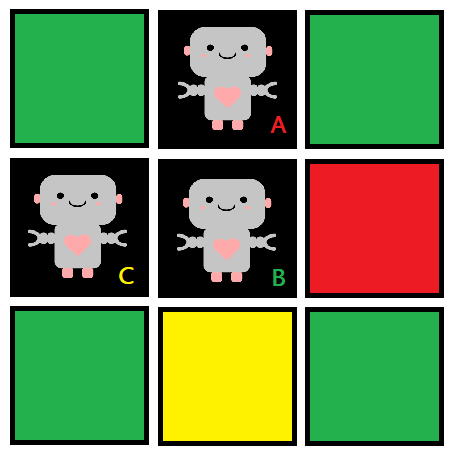
\includegraphics[scale=0.3]{robot_kinon.png}}
\end{center}

Pada gambar tersebut, robot A menyiram grid pada warna merah, robot B menyiram grid berwarna hijau, dan robot C menyiram grid berwarna kuning.

\end{document}